\documentclass[spanish,10pt,letterpaper, twocolumn]{article}
%\usepackage[utf8]{inputenc}
\usepackage{babel}
\usepackage{url}
\usepackage[lmargin=1.5in, rmargin=1in,tmargin=1in, bmargin=1in]{geometry}
\usepackage{amsmath}
\usepackage{amsfonts}
\usepackage{amssymb}
\usepackage{bm}
\usepackage{graphicx}
%\usepackage{subcaption}
\usepackage{float}
\usepackage[caption = false]{subfig}
\usepackage{listings}             % Incluye el paquete listings
\usepackage[T1]{fontenc}



\title{Tarea 01 -Posicionamiento de un robot movil-}
\author{Rob\'otica, Ingenier\'ia Mecatr\'onica\\
Instituto de Ingenier\'ia y Tecnolog\'ia, UACJ\\
Catedr\'atico: Dr. Edgar A. Martinez\\
%%%Nombre(s) Alumno(s)
\textbf{Jos\'e F\'elix Velazco Velazco}\\ 
\url{al140621@uacj.mx}
}
\date{\today}

\providecommand{\e}[1]{\ensuremath{\times 10^{#1}}}




\begin{document}
\maketitle

\section*{Abstract}
En este reporte se ver\'a el modelo de control para manejar un amigobot mediante el vector $\vec{\dot{u}}$, que contiene $v$ y $\omega$. Con esto hecho se obtendr\'a la posici\'on del robot mediante un sistema de visi\'on que se localiz\'o en el techo del laboratorio, esto lleva consigo el procesamiento de im\'agenes con el fin de obtener el mejor resultado posible. Adem\'as, tambi\'en se obtendr\'a la posici\'on odom\'etrica que ser\'a provista por el amigobot directamente.
\section{Modelo de generacion de trayectorias}
Para la trayectoria a seguir del robot, se opt\'o por tomar una funci\'on $y(x)=\sin(x)$. La trayectoria a seguir debe de tener una amplitud de -0.8 a 0.8, y que se complete una onda completa empezando de 0 a 2, por lo que la funci\'on $y(x)$ como se ve en la ecuaci\'on \eqref{eq:eq1}.

\begin{equation}
{
	\label{eq:eq1}
	y(x)=0.8\cdot \sin\left( \frac{2\pi}{x^{max}}\cdot x\right) 
}
\end{equation}

Donde $x^{max}$ ser\'a la distancia m\'axima de la onda, en este caso es igual a 2.
Se obtuvieron 1000 valores de $x$, de 0 a 2 con incrementos de 0.002\\
y con estos valores se calcularon los valores de $y(x)$ y teniendo estos valores en una tabla, se obtuvieron $\dot{x}$ y $\dot{y}$, mediante derivadas num\'ericas, obteniendo las ecuaciones \eqref{eq:eq2} y \eqref{eq:eq3} para obtener nuevamente 1000 valores

\begin{equation}
	\label{eq:eq2}
	\dot{x}=\frac{dx}{dt}=\frac{x_t-x_{(t-1)}}{\Delta t}
\end{equation} 

\begin{equation}
	\label{eq:eq3}
	\dot{y}=\frac{dy}{dt}=\frac{y_t-y_{(t-1)}}{\Delta t}
\end{equation} 

Con estos valores, se obtuvieron los valores de $\dot{s}$ y $\theta$ con las ecuaciones \eqref{eq:eq4} y \eqref{eq:eq5}.

\begin{equation}
	\label{eq:eq4}
	\dot{s}=\sqrt{\dot{x}^2+\dot{y}^2}
\end{equation} 

\begin{equation}
	\label{eq:eq5}
	\theta=\arctan\left(\frac{\dot{y}}{\dot{x}}\right)	
\end{equation}

Al obtener los valores de $\dot{s}$ y $\theta$, estos valores se meter\'an en una regresi\'on de grado 7, 

Se sabe que $y=A \cdot x$, al despejar x, obtendremos la soluci\'on inversa $x=A^{-1} \cdot y$. En la ecuaci\'on \eqref{eq:eq6} se puede ver en su forma matricial, donde $y_i$ se sustituir\'a por $\dot{s}_i$ y $\theta_i$. 

\begin{equation}
\label{eq:eq6}
\begin{bmatrix}
	a_0 \\
	a_1 \\
	\vdots \\
	a_7
\end{bmatrix}
	=
\begin{bmatrix}
	N & \Sigma t  & \cdots & \Sigma t^7\\
	\Sigma t & \Sigma t^2  & \cdots & \Sigma t^8\\
	\vdots & \vdots & \ddots & \vdots \\
	\Sigma t^7 & \Sigma t^8 & \cdots & \Sigma t^{14}
\end{bmatrix} ^{-1}
\cdot
\begin{bmatrix}
	\Sigma(y_i)\\
	\Sigma(t_iy_i)\\
	\vdots \\
	\Sigma(t_i^7y_i)
\end{bmatrix}
\end{equation}

Esta operaci\'on nos dar\'a los polinomios de $v(t)=\dot{s}(t)$ y $\theta(t)$.

\begin{equation}
	\label{eq:eq7}
	\begin{matrix}
	v(t)=-4.19\e{-5}+0.02t-0.005t^2\\
	+5.88\e{-4}t^3-3.17\e{-5}t^4\\
	+8.35\e{-7}
t^5-8.57\e{-9}t^6
	\end{matrix}
\end{equation}

\begin{equation}
	\label{eq:eq8}
	\begin{matrix}
	\theta(t)=-9.52\e{-5}+0.06t-0.015t^2\\
	+0.0013t^3-5.89\e{-5}t^4+1.41\e{-6}t^5\\
	-1.43345\e{-8}t^6
	\end{matrix}
\end{equation}

Se tiene la velocidad lineal $v(t)$ como se ve en la ecuaci\'on \eqref{eq:eq7}. Para la velocidad angular, solo derivamos el polinomio $\theta(t)$, que se ve en la ecuaci\'on \eqref{eq:eq8}, para obtener finalmente $\omega (t)$ 
 
\begin{equation}
	\label{eq:eq9}
	\begin{matrix}
		\omega (t)=0.06-0.029t+0.004t^2-2.4\e{-4} t^3 \\
		 +7.076\e{-6}t^4-8.6\e{-8}t^5
	\end{matrix}
\end{equation}


\begin{figure}[ht]
	\centering
	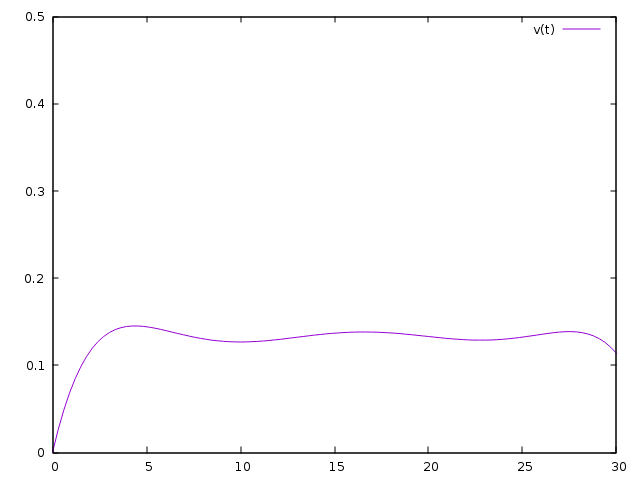
\includegraphics[scale=0.2]{v.png}
	\caption{Gr\'afica de la velocidad lineal $v(t)$}
	\label{modelo:fig1}
\end{figure}

\begin{figure}[ht]
	\centering
	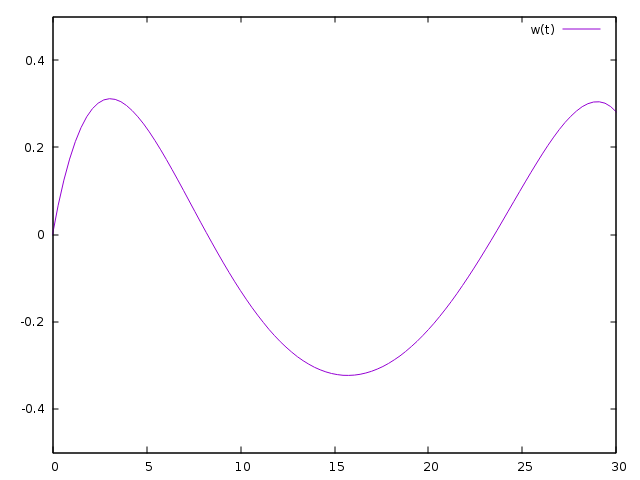
\includegraphics[scale=0.2]{w.png}
	\caption{Gr\'afica de la velocidad angular $\omega(t)$}
	\label{modelo:fig2}
\end{figure}
	
En las figuras \ref{modelo:fig1} y \ref{modelo:fig2} se pueden observar el comportamiento de estas velocidades.

%%%%%%%%%%%%%
%%Las secciones del reporte tendran el titulo mas idoneo posible. No existe un numero para el total de secciones.
\section{Modelo odom\'etrico}
Para esta secci\'on, se utilizar\'a un modelo de 3 ruedas, donde una actua como \textit{steer}, y las otras dos como \textit{drive}, tal y como se muestra en la figura \ref{fig:fig1}

\begin{figure}[ht]
\centering
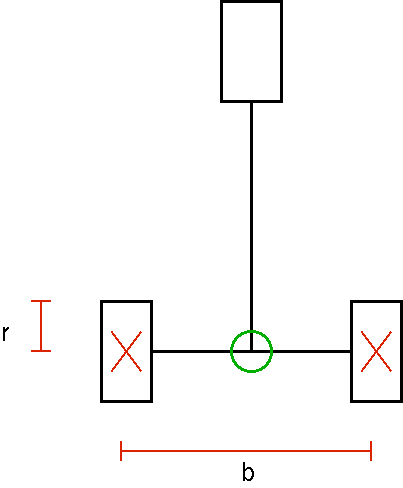
\includegraphics[scale=0.2]{carro.png}
\caption{Esquema b\'asico del amigobot}
\label{fig:fig1}
\end{figure}



\subsection{Od\'ometros}
Tomando en cuenta que el amigobot sensa mediante encoders, entonces se obtiene el siguiente modelo

\begin{equation}
	\label{eq:eq10}
	s=\frac{2\pi r}{R}* \eta
\end{equation}

Con una derivada num\'erica sacamos las velocidades de cada llanta, as\'i como se ve en la ecuaci\'on \eqref{eq:eq12}

\begin{equation*}
	\label{eq:eq11}
	v_D=\frac{2\pi r}{R \Delta t}(\eta_{R2}-\eta_{R1})
\end{equation*}

\begin{equation}
	\label{eq:eq12}
	v_L=\frac{2\pi r}{R \Delta t}(\eta_{L2}-\eta_{L1})
\end{equation}

La velocidad lineal del amigobot ser\'ia el promedio de las velocidades de las llantas. Y a partir de la ecuaci\'on \eqref{eq:eq13}, podemos inferir un modelo en donde se vean implicados las velocidades angulares de las llantas, como en la ecuaci\'on \eqref{eq:eq14}.


\begin{equation}
	\label{eq:eq13}
	v_t=\frac{V_R+V_L}{2}
\end{equation}

\begin{equation*}
	v_{(R,L)}=r \varphi_{(R,L)}
\end{equation*}

\begin{equation*}
	\therefore v_t=\frac{r\dot{\varphi}_R+r\dot{\varphi}_L}{2}
\end{equation*}

\begin{equation}
	\label{eq:eq14}
	v_t(\dot{\varphi}_R,\dot{\varphi}_L)=\frac{r}{2}(\dot{\varphi}_R+\dot{\varphi}_L)
\end{equation}

Ahora obtendremos el modelo de velocidad angular en funci\'on de las velocidades angulares de las llantas, asumiendo que 

\begin{equation}
	\label{eq:eq15}
	\hat{v}_t=v_R-v_L
\end{equation}

Entonces, tendremos que

\begin{equation}
	\label{eq:eq16}
	\omega_t=\frac{\hat{v}_t}{\frac{b}{2}}=\frac{2}{b}\hat{v}_t
\end{equation}

\begin{equation}
	\label{eq:eq17}
	\omega_t(\dot{\varphi}_R,\dot{\varphi}_L)=\frac{2r}{b}(\dot{\varphi}_R-\dot{\varphi}_L)
\end{equation}

Y con la ecuaci\'on \eqref{eq:eq14} y \eqref{eq:eq17}, ser\'a nuestra ley de control.

\subsection{Cinem\'atica}

A partir de nuestra ley de control, vista en el tema pasado, podemos describirlo de manera matricial. 

\begin{equation}
	\label{eq:eq18}
	\begin{bmatrix}
		v_t \\ \\
		w_t
	\end{bmatrix}
	=
	\begin{bmatrix}
		\frac{r}{2} & \frac{r}{2} \\ \\
		\frac{2r}{b} & \frac{2r}{b}
	\end{bmatrix}
	\cdot
	\begin{bmatrix}
		\dot{\varphi}_R \\ \\
		\dot{\varphi}_L
	\end{bmatrix}
\end{equation} 

Para obtener nuestro vector de control, as\'i como se ve en la ecuaci\'on \eqref{eq:eq18}, tendremos que nuestra matriz de restricci\'on cinem\'atica lo multiplicaremos por nuestro vector de variables de control independiente, las cuales son las velocidades angulares de las llantas. 

Esto se hace cuando se conocen las velocidades angulares de las llantas, pero se desconoce el valor las velocidades $v_t$ y $\omega_t$. 

En caso de que si sepamos las velocidades $v_t$ y $\omega_t$, pero no las velocidades $\dot{\varphi}_R$ y $\dot{\varphi}_L$, entonces se opta por la soluci\'on inversa, con lo que tendriamos:

\begin{equation}
	\label{eq:eq19}
	\begin{bmatrix}
		\dot{\varphi}_R \\ \\
		\dot{\varphi}_L
	\end{bmatrix}
	=
	\begin{bmatrix}
		\frac{r}{2} & \frac{r}{2} \\ \\
		\frac{2r}{b} & \frac{2r}{b}
	\end{bmatrix}^{-1}
	\cdot
	\begin{bmatrix}
		v_t \\ \\
		w_t
	\end{bmatrix}
\end{equation} 

 
%%%%%%%%%%%%%%%%%%%%%%%%%%%%%%%%%%%%%%%%%%%%%%%%%%%%%%%%%%%%%%%%%%%


\section{Modelo de sensado visual}
\subsection{Posicionamiento de la c\'amara}
La labor de calibraci\'on de la c\'amara, es una parte fundamental al momento de querer utilizar un sistema de referencia global, esto es debido a que si no se calibra adecuadamente, de nada servir\'ia lo dem\'as de visi\'on.

Se puso la c\'amara en un sitio lo m\'as horizontal posible, y en una pared lo m\'as ortogonal posible a este plano, se pusieron unas marcas del campo de vision.

Para calcular los angulos $\varphi_{Horizontal}$ y $\varphi_{Vertical}$, del campo de visi\'on, se acomod\'o la c\'amara, as\'i como se ve en la figura \ref{vision:fig1}.


\begin{figure}[ht]
		\centering
		\subfloat[Vista superior]{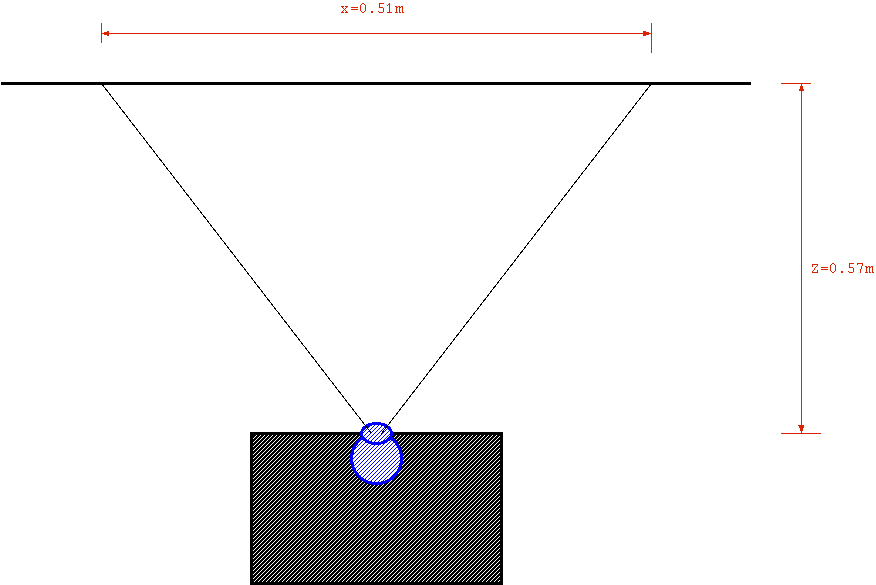
\includegraphics[scale=0.2]{camaraXZ.png}}\\
		\subfloat[Vista lateral]{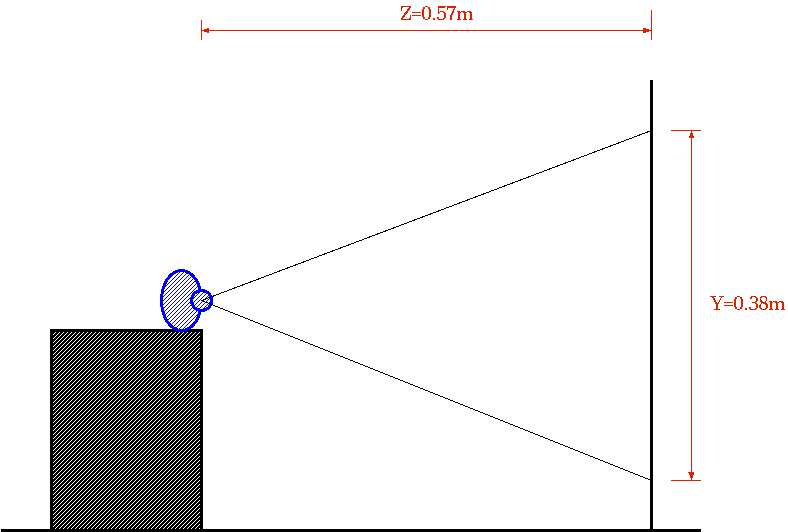
\includegraphics[scale=0.2]{camaraYZ.png}}
		\caption{Vistas del experimento para obtenci\'on del campo de visi\'on.}
		\label{vision:fig1}
\end{figure}

\begin{equation*}
	\varphi_H=2\arctan\left(\frac{x}{2z}\right)
\end{equation*}

\begin{equation}
	\label{vision:eq1}
	\varphi_v=2\arctan\left(\frac{y}{2z}\right)
\end{equation} 

Las ecuaciones \eqref{vision:eq1}, muestran la manera de calcular los angulos de campo de visi\'on que posee la c\'amara, las cuales, sustituyendo los valores, tendr\'iamos.

\begin{equation*}
	\begin{matrix}
	\varphi_H=2\arctan\left(\frac{0.51}{2(0.57)}\right)	\\
	\varphi_V=2\arctan\left(\frac{0.38}{2(0.57)}\right)		
	\end{matrix}
\end{equation*}
Obteniendo entonces los valores vistos en la ecuaci\'on \eqref{vision:eq2}
\begin{equation}
	\label{vision:eq2}
	\varphi_H=48.21^{\circ} \ ,	\ \ \varphi_V=36.87^{\circ}
\end{equation}

Despu\'es de esto, se localiz\'o la c\'amara en el techo, con el fin de abarcar el mayor campo de visi\'on posible. Al estar completamente calibrada, se obtuvo que la altura $z=2.74m$ desde el lente de la c\'amara hasta la marca del amigobot, donde el amigobot estaba en el centro del campo de visi\'on, tal y como se ve en la figura \ref{vision:fig2} 

\begin{figure}[ht]
	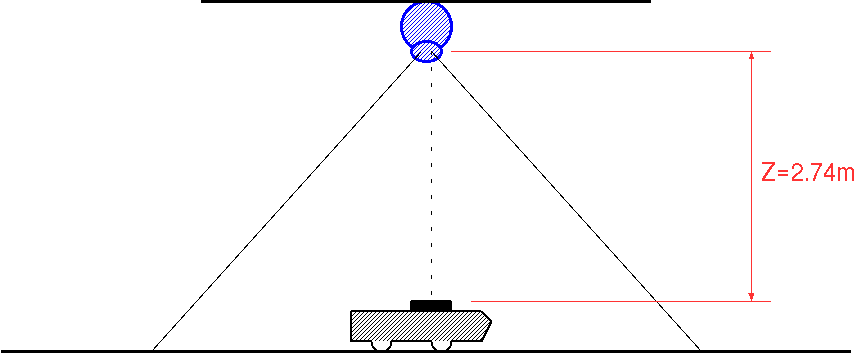
\includegraphics[scale=0.2]{global.png}
	\caption{Localizaci\'on de la c\'amara para el sistema de visi\'on global}
	\label{vision:fig2}
\end{figure}

De las ecuaciones \eqref{vision:eq1}, podemos despejar para obtener los valores $X$ y $Y$

\begin{equation}
	\begin{matrix}
		X=2z\tan\left(\frac{\varphi_H}{2}\right)=2(2.74)\tan\left(\frac{48.21}{2} \right)   \\ \\
		Y=2z\tan\left(\frac{\varphi_V}{2}  \right)=2(2.74)\tan\left(\frac{36.87}{2} \right)  
	\end{matrix}
\end{equation}

\begin{equation}
	\begin{matrix}
		X=2.45m & Y=1.83m
	\end{matrix}
\end{equation}

Con los valores de $X$ y $Y$ podemos finalmente deducir cuanto ser\'ia equivalente en metros cada pixel. Tomando en cuenta que las im\'agenes que tomaremos son de 640x480 pixels, se puede deducir que:

\begin{equation}
	\label{vision:eq3}
	\begin{matrix}
		X_{pixel}=\frac{1_{pixels}(2.45m)}{640_{pixels}}=3.82mm \\ \\
		Y_{pixel}=\frac{1_{pixels}(1.83m)}{480_{pixels}}=3.82mm
	\end{matrix}
\end{equation}

Con los valores obtenidos en las ecuaciones \eqref{vision:eq3} podremos obtener la posici\'on m\'as adelante. Y con esto \'ultimo se procede a tomar las fotos de la trayectoria del amigobot antes vista.


%%%%%%%%%%%%%%%%%%%%%%%%%%%%%%%%%%%%%%%%%%%%%%%%%%%%%%%%%%%%%%%%%%%%%%%%%%
%%%%%%%%%%%%%%%%%%%%%%%%%%%%%%%%%%%%%%%%%%%%%%%%%%%%%%%%%%%%%%%%%%%%%%%%%%
%%%%%%%%%%%%%%%%%%%%%%%%%%%%%%%%%%%%%%%%%%%%%%%%%%%%%%%%%%%%%%%%%%%%%%%%%%


\subsection{Mejoramiento y filtrado}
Una vez tomada todas las im\'agenes, se procede a utilizar un tipo tipo de mejoramiento, cambiando el brillo y el contraste de estas. En la image \ref{vision:fig3} se puede observar la imagen original tomada por la c\'amara.

\begin{figure}[ht]
	\centering
	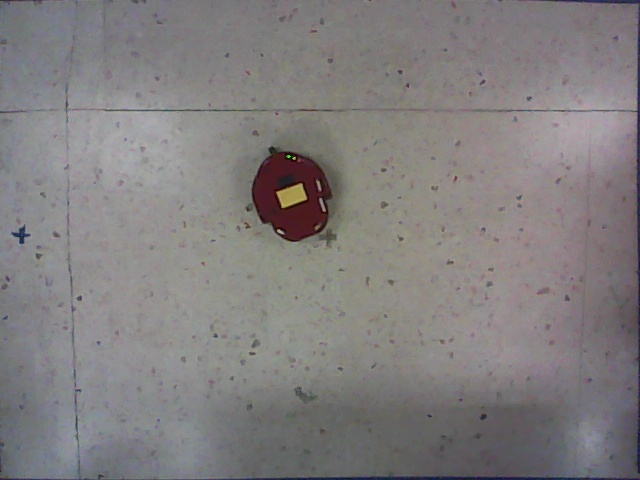
\includegraphics[scale=0.2]{foto150.jpg}
	\caption{Imagen original}
	\label{vision:fig3}
\end{figure}

\lstset{language=C++}
\begin{lstlisting}[frame=single]
src.convertTo(dst,-1, 3,10);

for ( int i = 1; i < M; i = i + 2 )
{
	medianBlur ( dst, dst, i );
}
\end{lstlisting}

En el c\'odigo anterior, se ve la funci\'on converTo, que lo que hace es modificar el brillo y el contraste, en este caso particular se opt\'o por darle un contraste de 3, y un brillo de 10.

\begin{figure}[ht]
	\centering
	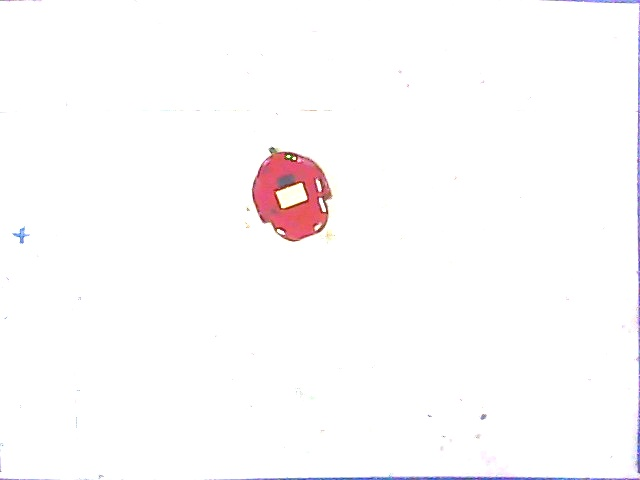
\includegraphics[scale=0.2]{median150.jpg}
	\caption{Imagen con mejoramiento y filtrado aplicado}
	\label{vision:fig4}
\end{figure}

La funci\'on medianBlur, lo que hace, es que aplica un filtro de mediana en la imagen, esto con el fin de suavizar m\'as los colores, en este caso, se utiliz\'o un kernel de 3x3.


\subsection{Filtrado Morfol\'ogico}
Para el filtrado morfol\'ogico, primero necesitamos convertir la imagen, en BGR, en una imagen binarizada, esto, se logra mediante la divisi\'on de la imagen orignal en 3 canales distintos: B,G,R. Con esto, dej\'andolo todo para segmentar el color amarillo elimindando el canal B. \\
Obtenida la imagen binarizada, aplicariamos el siguiente c\'odigo.

\lstset{language=C++}
\begin{lstlisting}[frame=single]
float morph_size = 4; 

Mat kernel = getStructuringElement
(MORPH_RECT, Size(2*morph_size+1, 
2*morph_size+1), Point(morph_size,
 morph_size) );


	erode(r, r, kernel);


morph_size = 4;

kernel = getStructuringElement
(MORPH_RECT, Size(2*morph_size+1,
2*morph_size+1), Point(morph_size, 
morph_size) );

	dilate(r, r, kernel);
\end{lstlisting}

Aqu\'i se debe de destacar m\'as que nada las funciones \textit{erode} y \textit{dilate}, la cual, la primera lo que hace es ir degradando los trozos peque\~nos que quedan por ah\'i esparcidos en la imagen binarizada. Una vez degradada, se procede a volver a su tama\~no original todos los dem\'as elementos con la funci\'on \textit{dilate}. En este caso se utilizo un kernel de 9x9. El resultado se puede apreciar en la figura \ref{vision:fig5}

\begin{figure}[ht]
	\centering
	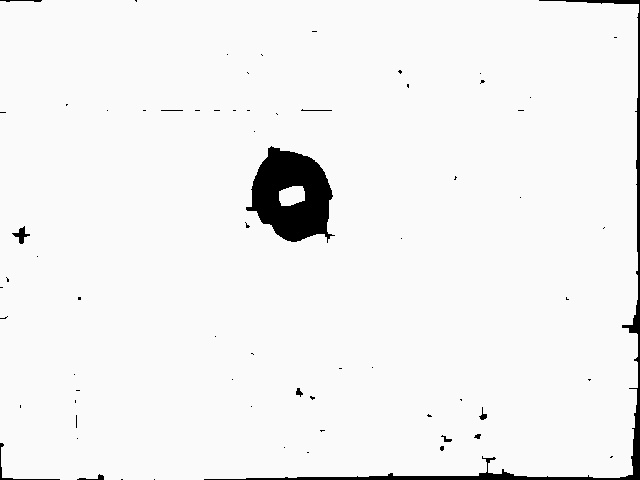
\includegraphics[scale=0.2]{filtrado150.jpg}
	\caption{Imagen  filtrada con operadores morfol\'ogicos}
	\label{vision:fig5}
\end{figure}

\subsection{Segmentaci\'on por etiquetado de componentes conectados}

\lstset{language=C++}
\begin{lstlisting}[frame=single]
Mat labels,stats, centroids;

int nLabels = 
connectedComponentsWithStats
(r, labels, stats, centroids,8,
 CV_16U);
	
int z=0;
for(z=0; z<nLabels;z++)
{
	int area=0, temp=0;
	area=stats.at<int>(z,4);
	if(area>320 && area<500) 
		break;
}
float x= centroids.at<double>(z,0);
float y= centroids.at<double>(z,1);
\end{lstlisting}

La funci\'on \textit{connectedComponentsWithStats}() es la funci\'on que nos ayuda a poder aplicar el modelo de segmentaci\'on por etiquetado de componentes conectados, que a su vez, nos puede proporcionar datos como el \'area, o el centroide del objeto, por lo que con esto, se pudo obtener lo que se muestra en la figura \ref{vision:fig6} 

\begin{figure}[ht]
	\centering
	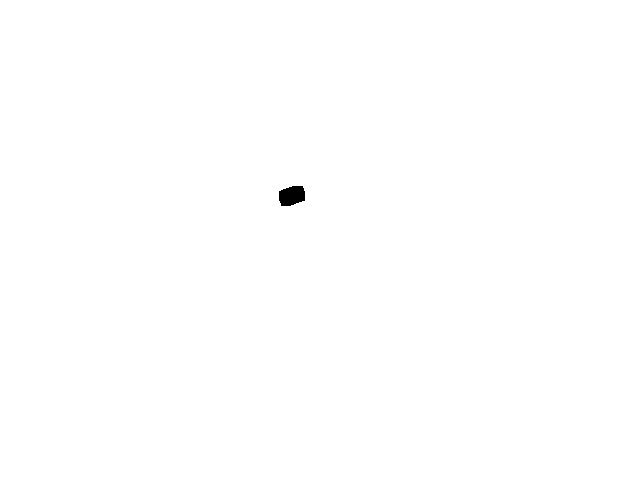
\includegraphics[scale=0.16]{labels150.jpg}
	\caption{Marca segmentada (en negativo)}
	\label{vision:fig6}
\end{figure}




\subsection{Modelo de visi\'on 3D}
Para el modelo de visi\'on 3D, se tuvo que obtener el centroide de la marca durante todo el recorrido del amigobot, el cual se puede obtener mediante la funci\'on vista anteriormente  \textit{connectedComponentsWithStats}()

Los valores de $x$ y $y$ est\'an dados en pixeles, por lo que se debe de pasar convertir a metros.

\lstset{language=C++}
\begin{lstlisting}[frame=single]
float x= centroids.at<double>(z,0);
float y= centroids.at<double>(z,1);

float x1=0.0, y1=0.0;
x1=((x-320)*3.82*pow(10,-3));
y1=((-y+240)*3.82*pow(10,-3));

B(i,0)=x;
B(i,1)=y;
\end{lstlisting}

$x_1$ y $y_1$ ser\'ia la distancia en metros, mientras que $x$ y $y$ es\'a dada en pixels, por lo que primero, movemos el origen que viene por default localizado en la ezquina superior izquierda, en (320,-240). Una vez hecho esto, multiplicamos el pixel dado por $3.82\times 10^{-3}$ que es la equivalencia en metros de cada pixel, obteniendo as\'i la posici\'on del sistema de visi\'on global, como se aprecia en la figura \ref{vision:fig7}


\begin{figure}[ht]
	\centering
	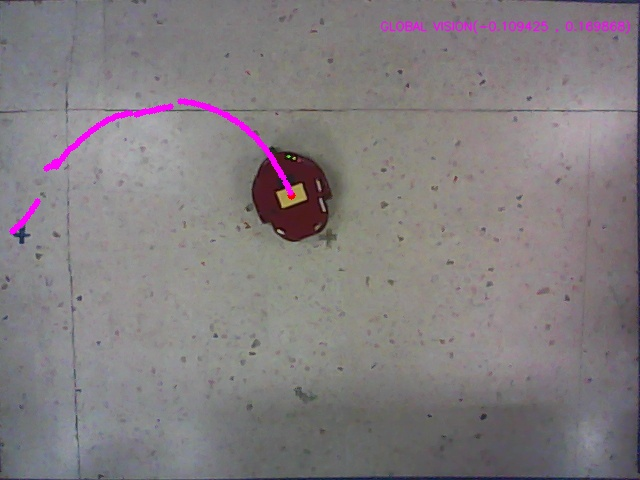
\includegraphics[scale=0.3]{mejora150.jpg}
	\caption{Sistema global de visi\'on}
	\label{vision:fig7}
\end{figure}

\section{Resultados}

Las posiciones cartesianas se pueden observar en la figura \ref{resultados:fig1}

\begin{figure}[ht]
	\centering
	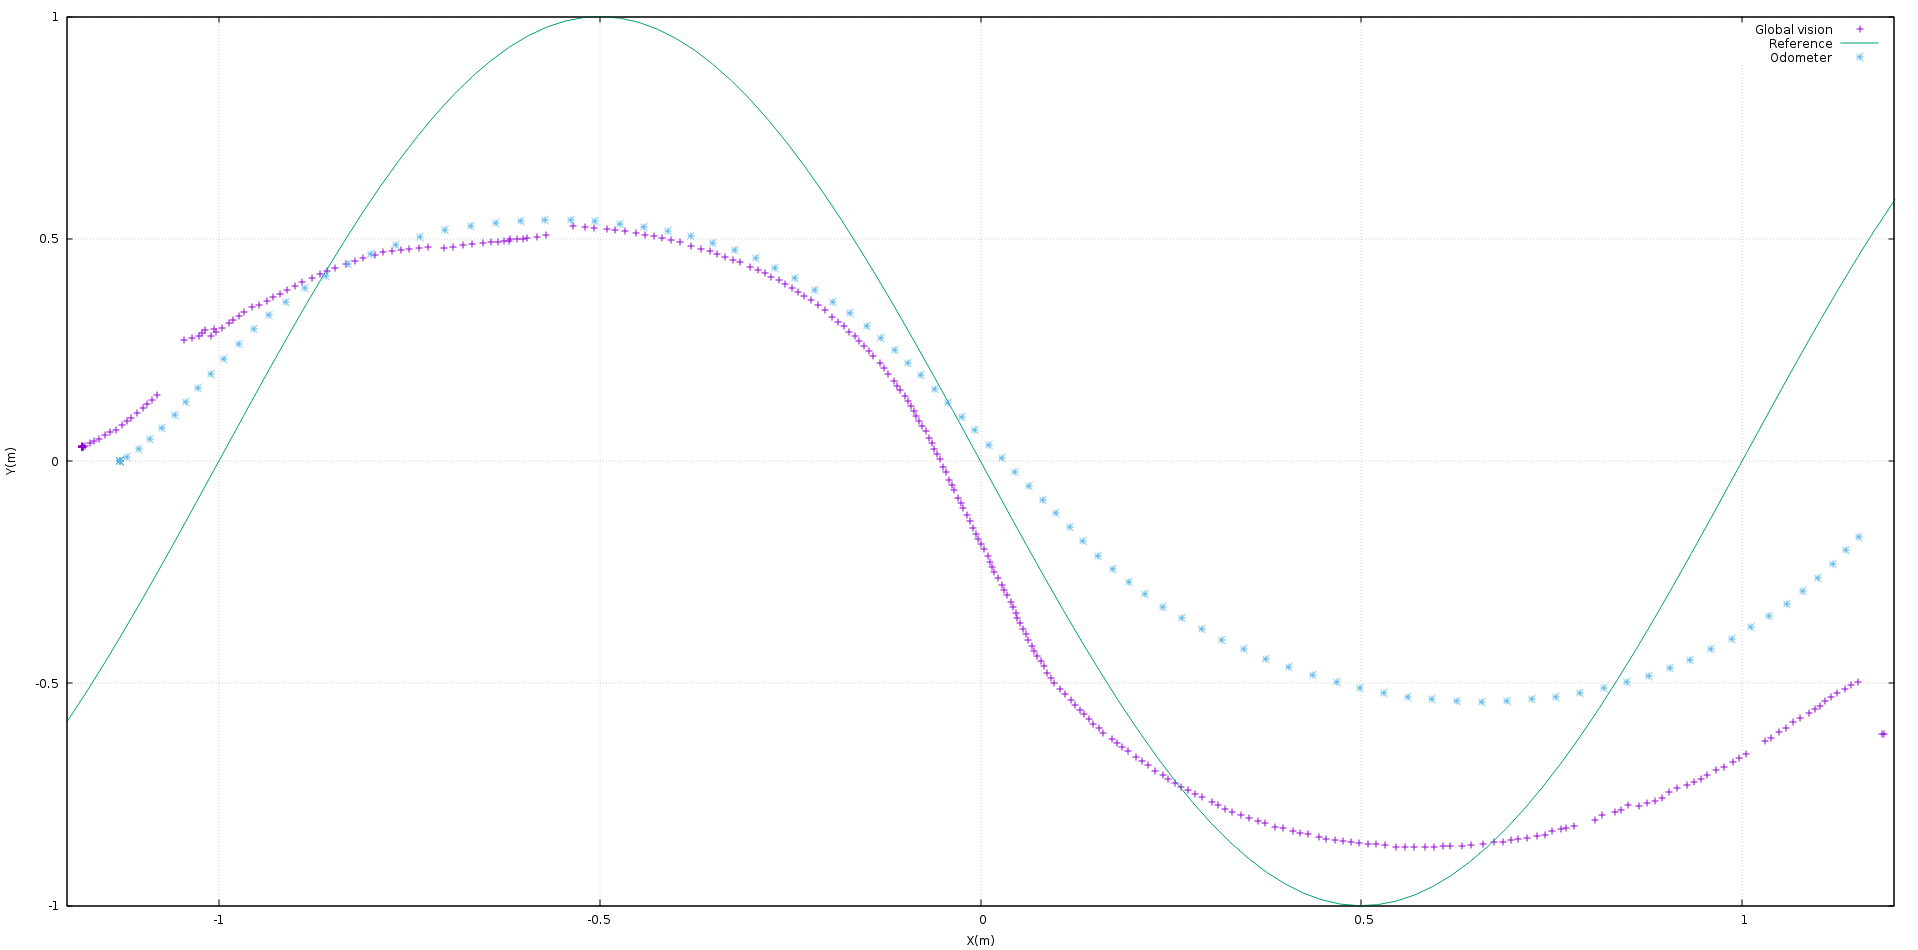
\includegraphics[scale=0.15]{graficas.png}
	\caption{Gr\'afica de la posici\'on cartesiana seg\'un el valor de referencia, la visi\'on global, y la odometr\'ia}
	\label{resultados:fig1}
\end{figure}

Las trayectorias tambi\'en se pueden ver en la imagen \ref{resultados:fig2}, junto con la imagen del amigobot.
\begin{figure}[ht]
	\centering
	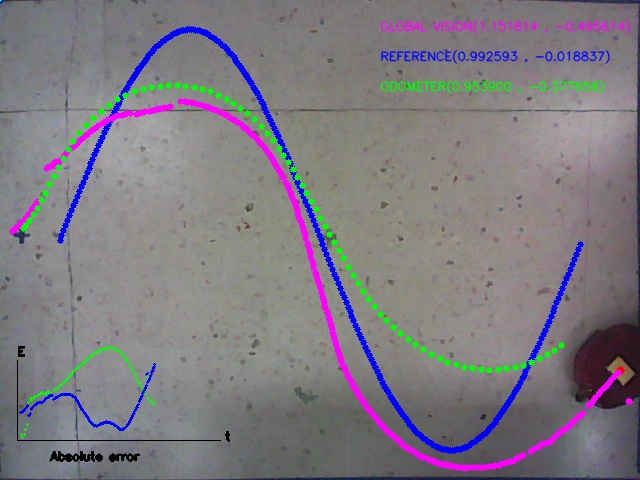
\includegraphics[scale=0.2]{mejora309.jpg}
	\caption{Recorrido del amigobot seg\'un: la odometr\'ia, la visi\'on global, y la referencia}
	\label{resultados:fig2}
\end{figure}

\subsection{Error absoluto y relativo}
En base de las ecuaciones \eqref{resultados:eq1} y \eqref{resultados:eq2}, que se ven a continuaci\'on:

\begin{equation}
	E_a=\left| \vec{P}_V - \vec{P}_R  \right|
	\label{resultados:eq1}
\end{equation}

\begin{equation}
	E_r=\left| \frac{\vec{P}_V - \vec{P}_R}{\vec{P}_V}  \right|
	\label{resultados:eq2}
\end{equation}

Se puede sacar las gr\'aficas de los errores absolutos de \textit{Visi\'on  vs Odometria} y de \textit{Visi\'on vs Referencia}.

\begin{figure}[ht]
	\centering
	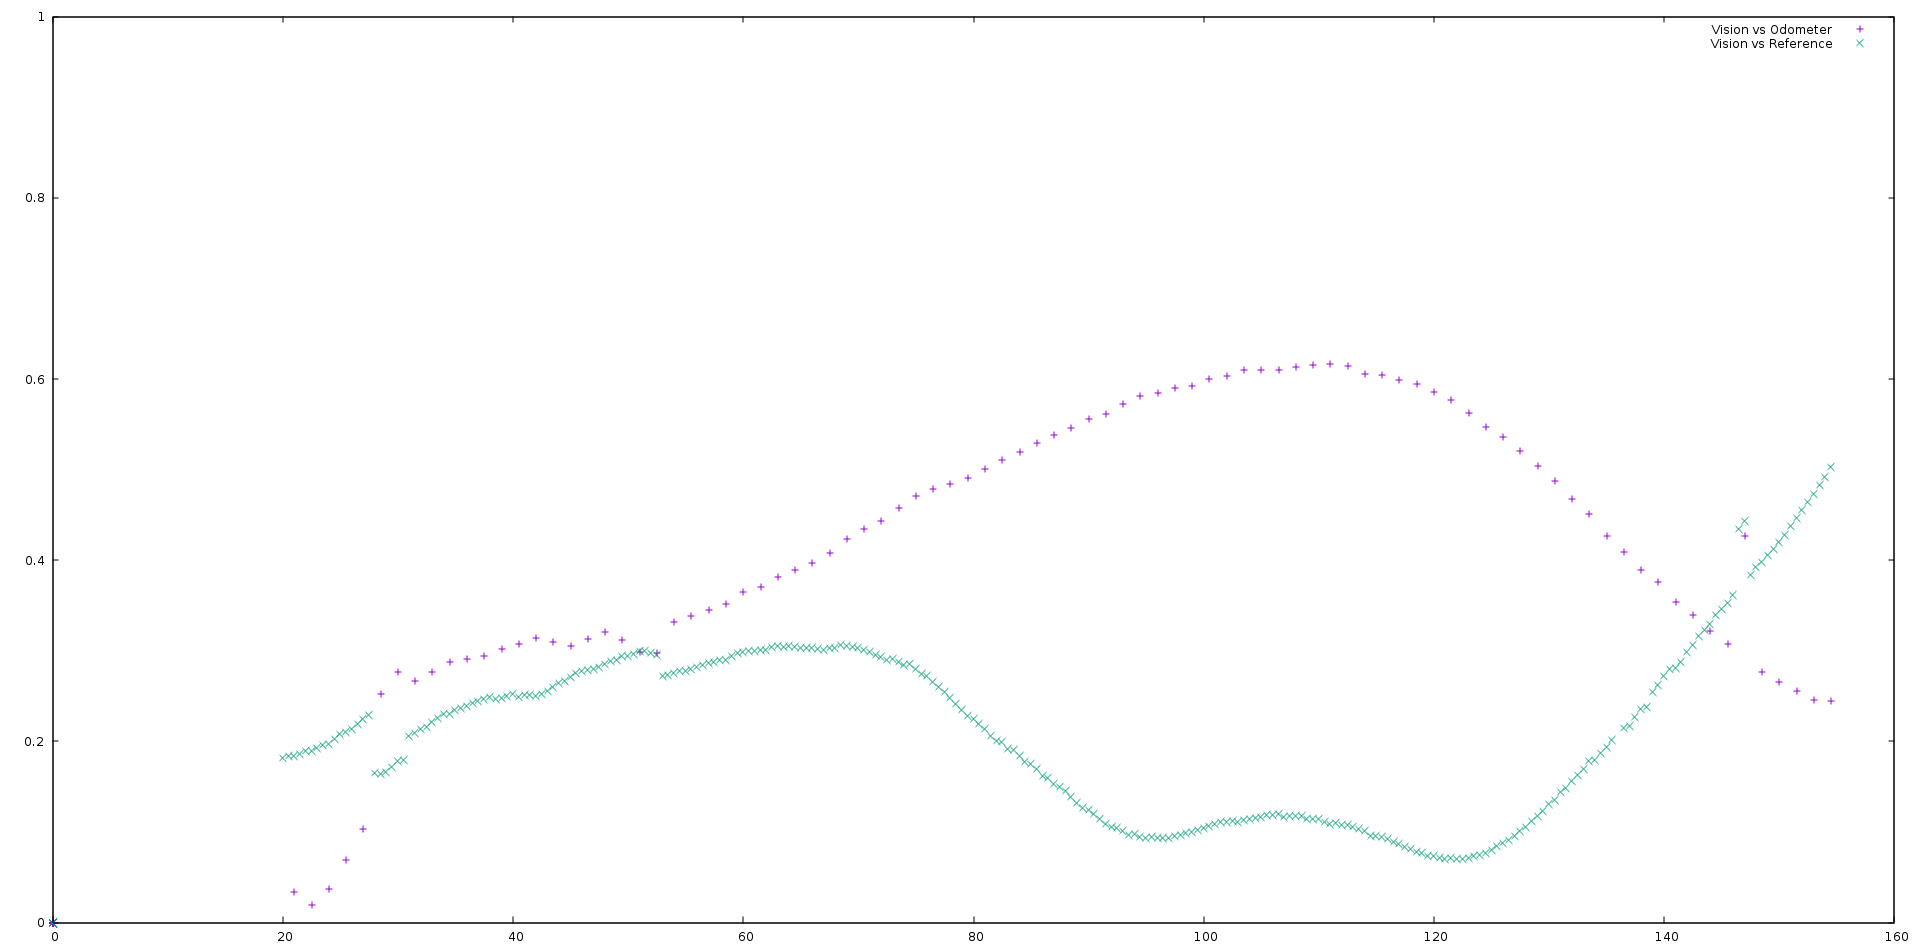
\includegraphics[scale=0.11]{errorAbsoluto.png}
	\caption{Gr\'afica del error absoluto de \textit{Visi\'on  vs Odometria} y de \textit{Visi\'on vs Referencia}}
	\label{resultados:fig3}
\end{figure}

\begin{figure}[ht]
	\centering
	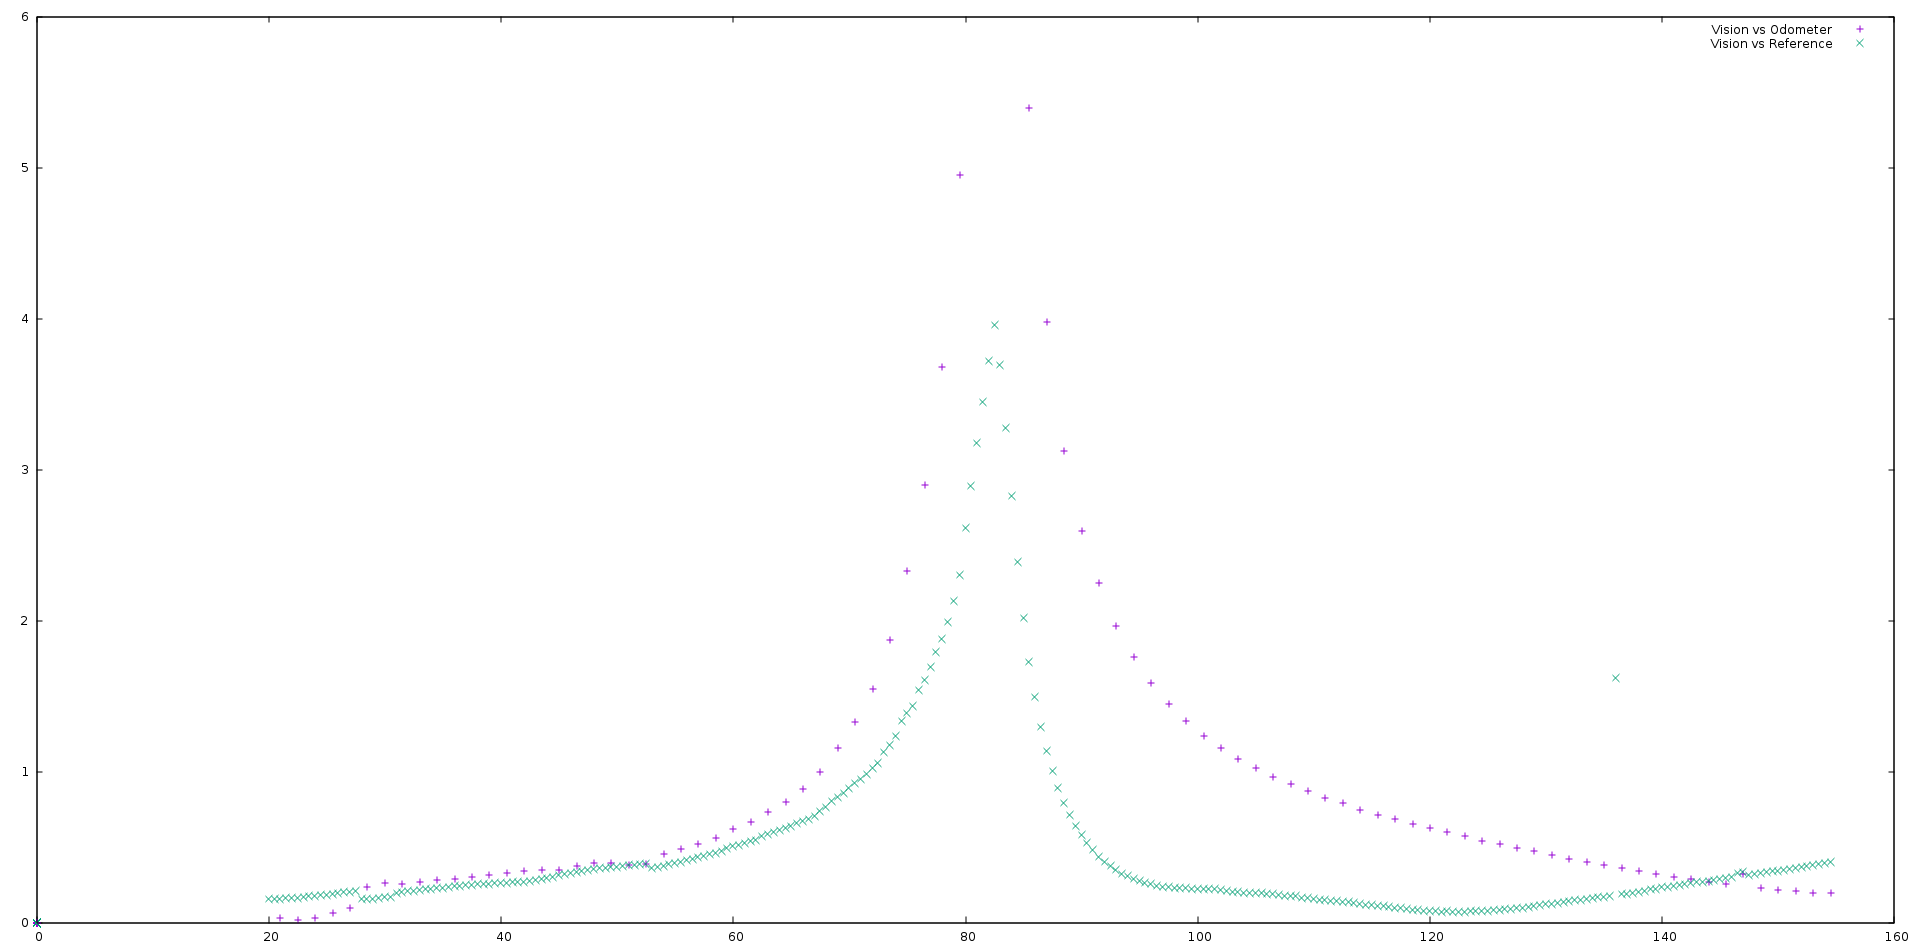
\includegraphics[scale=0.11]{errorRelativo.png}
	\caption{Gr\'afica del error relativo de \textit{Visi\'on  vs Odometria} y de \textit{Visi\'on vs Referencia}}
	\label{resultados:fig4}
\end{figure}
 

\section{Conclusiones}
Al final se logr\'o cumplir con los requerimientos encomendados. Hubo una dificultad grande al tratar de conseguir el vector de control $\vec{\dot{u}}$, pero se logr\'o hallar el error en la programaci\'on que finalmente resolvi\'o ese problema.

\begin{equation}
		\omega (t)=0.06-0.029t+0.004t^2-2.4\e{-4} t^3 
		 +7.076\e{-6}t^4-8.6\e{-8}t^5
\end{equation}


\begin{equation}
	y(x)=\pi x-\frac{\pi ^3}{6}x^3+\frac{\pi ^5}{120}x^5-\frac{\pi ^7}{5040}x^7
\end{equation}


\begin{equation}
\omega(t)=-9.52\e{-5}+0.06t-0.015t^2
	+0.0013t^3-5.89\e{-5}t^4+1.41\e{-6}t^5
	-1.43345\e{-8}t^6
\end{equation}

\begin{equation}
	v(t)=-4.19\e{-5}+0.02t-0.005t^2
	+5.88\e{-4}t^3-3.17\e{-5}t^4
	+8.35\e{-7}
t^5-8.57\e{-9}t^6
\end{equation}

\end{document}

